\section{Channel System}
\label{sec:channelSystem}

With each member being a set of roles, it remains to model a description of how each member communicates with another, exchanging information during the mission. Recalling our motivation example, some requirements are still missing, and need to be addressed. First, during the entire mission, members are communicating with some other entity all the time. This means that parallelism is important to maintain each entity executing its roles, i.e, functionalities, at the same time. For instance, drones that only execute tasks in some particular C2 approach can communicate with the drone that detains the task allocator role, while executing the next task. Most importantly, the drone responsible for allocating tasks can use some protocol to assess the status of the members, e.g, checking if the drone dropped or is fully functional. Likewise, the C2 approach selector and task allocator roles can exchange messages that may cause a new maneuver, caused by context changes.

A channel system is composed of a group of data-dependent processes communicating with each via \textit{communication actions}~\cite{modelcheckingBaier}. With a program graph representing each process, transitions can be classified between conditional transitions, functioning as explained in Section \ref{subsec:PG}, or communication actions. This last type of transition works transmitting values through channels or receiving values from channels and assigning them to variables~\cite{modelcheckingBaier}. Additionally, channels can have a finite or infinite capacity of messages in a single channel, as well as a specified type of messages that can be stored in it. Finally, channel systems provide a notion of synchronization, whereas channels with a capacity different from zero function in a \textit{asynchronous} way and null capacity channels represent \textit{synchronous} communication~\cite{modelcheckingBaier}.

In our motivating example, each member, comprising a set of role's program graphs, is switching between actions related to its function or actions related to communication purposes. To decide which action to take, members update variables to properly evaluate conditions. Thus, when a condition related to some context change becomes true, the member can transmit this feedback to the member that possesses the task allocator role using, for example, the channel \textit{ch1}. If the task allocator decides that the current C2 Approach is not capable of maintaining quality during execution, it can send a maneuver request to C2 approach selector drone, using, for example, channel \textit{ch3}. Figure \ref{fig:CS} illustrates this scenario.

%%%%%%%%%%%%%%%%%%%%%%%%%%%%%%%%%%%

To provide C2 Agility, we present a computational model capable of representing the scenario elements behaviour based on the roles that such elements have. To cope with context changes, i.e., to provide C2 Agility, these members must reconfigure themselves or adjust their coordination through the communication structure and information exchanging. This capacity is demonstrated through a model that allows data exchange, so called channels, and a members' architecture  composed by features that can be enabled according to the circumstances, generating different configurations.

The proposed computational model is a typed-parameterized extension of the channel system defined by~\cite{MC01}, henceforth referred to as C2 channel system (C2CS). This proposal is based on the principles of Channel Systems formed by PG, besides the modeling of the domain entities as Dynamic Software Products that allows the possibility of re-configuring according to circumstances, activating features compatible with the tasks to be performed by such entities, so called members.



\subsection{Typed-Parameterized Channel System}
\label{sec:channelSystem}


Essentially, C2CS defines coordination among entities and their reconfiguration to cope with context changes eventually arising during a mission. These behaviors are described by three different program graphs (PGs) making up C2CS and representing role types played by entities: \textit{Executor (EX)}, \textit{Task Allocator (TA)}, and \textit{C2 approach selector (C2A)}. EX establishes task execution and reconfiguration behavior. TA defines task allocation responsibilities, and C2A specifies a C2 approach change protocol. 

The use of CS allows the execution of parallel processes in a system. Such structure allows us to put the identified papers in parallel execution and allows the exchange of information between them. This exchange is possible through the buffers, i.e., channels, used by the communication actions defined in CS modelling. [[In a nutshell, a CS can be represented as a set of Transition Systems, being each one corresponding to the unfold of each PG in CS. Such principle has a large application in Self Adaptive Systems using automata and Autonomous Systems.]

Given the scope of the research problem, C2CS leverages parameters to abstract from specific mission, entities, and initial conditions. For a particular mission with $n$ members in the team, there will  be only one instance of both the C2A and the TA roles, but $n$ EX instances. The member-to-role-instance mapping is such that each team member plays each EX role instance, and it contributes \textit{partially} to both the TA and the C2A roles, the amount of such contribution depending on the current C2 approach. Conversely, each EX role instance is cohesively encapsulated in one member, whereas the C2A and the TA roles are \textit{scattered} throughout team members, given the inherent collaborative nature of these roles. Types are used to describe the structure of the state of the different PGs as well as of the message content exchanged in synchronous and asynchronous channels.
Figure \ref{fig:cs} depicts C2CS, whereas Equation~\ref{eq:cs} defines it.

\begin{figure}[!ht]
    \centering
    \scalebox{.75}{

\tikzset{every picture/.style={line width=0.75pt}} %set default line width to 0.75pt        

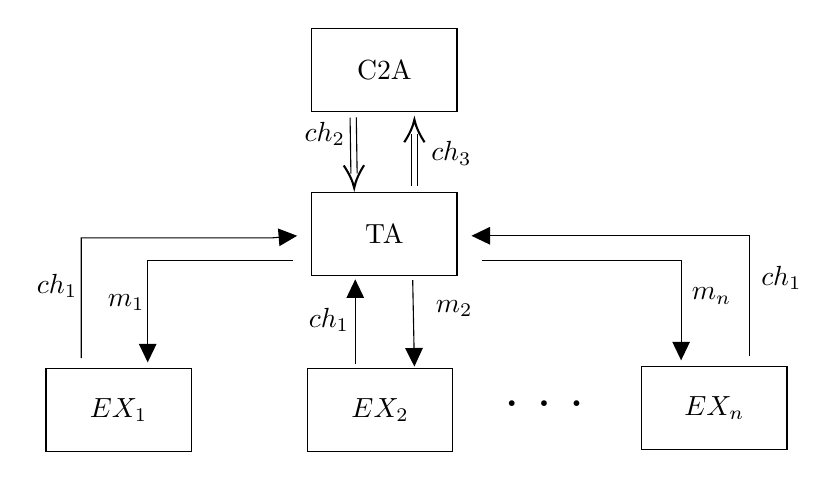
\begin{tikzpicture}[x=0.75pt,y=0.75pt,yscale=-1,xscale=1]
%uncomment if require: \path (0,225); %set diagram left start at 0, and has height of 225

%Shape: Rectangle [id:dp7793135649662085] 
\draw   (146,89) -- (216,89) -- (216,129) -- (146,129) -- cycle ;
%Shape: Rectangle [id:dp8388066725390221] 
\draw   (146,10) -- (216,10) -- (216,50) -- (146,50) -- cycle ;
%Shape: Rectangle [id:dp48691256180587716] 
\draw   (18,174) -- (88,174) -- (88,214) -- (18,214) -- cycle ;
%Straight Lines [id:da7136052167478543] 
\draw    (194.67,131.33) -- (195.44,170) ;
\draw [shift={(195.5,173)}, rotate = 268.85] [fill={rgb, 255:red, 0; green, 0; blue, 0 }  ][line width=0.08]  [draw opacity=0] (8.93,-4.29) -- (0,0) -- (8.93,4.29) -- cycle    ;
%Straight Lines [id:da1199439366931846] 
\draw    (35,169) -- (35,111) -- (127,111) -- (136.01,110.25) ;
\draw [shift={(139,110)}, rotate = 535.24] [fill={rgb, 255:red, 0; green, 0; blue, 0 }  ][line width=0.08]  [draw opacity=0] (8.93,-4.29) -- (0,0) -- (8.93,4.29) -- cycle    ;
%Shape: Rectangle [id:dp8070909053866772] 
\draw   (305,173) -- (375,173) -- (375,213) -- (305,213) -- cycle ;
%Shape: Rectangle [id:dp18131918632628874] 
\draw   (144,174) -- (214,174) -- (214,214) -- (144,214) -- cycle ;
%Straight Lines [id:da23459308482895536] 
\draw    (357,168) -- (357,110) -- (226,110) ;
\draw [shift={(223,110)}, rotate = 360] [fill={rgb, 255:red, 0; green, 0; blue, 0 }  ][line width=0.08]  [draw opacity=0] (8.93,-4.29) -- (0,0) -- (8.93,4.29) -- cycle    ;
%Straight Lines [id:da9340034396500284] 
\draw    (228,122) -- (324,122) -- (324,167) ;
\draw [shift={(324,170)}, rotate = 270] [fill={rgb, 255:red, 0; green, 0; blue, 0 }  ][line width=0.08]  [draw opacity=0] (8.93,-4.29) -- (0,0) -- (8.93,4.29) -- cycle    ;
%Straight Lines [id:da26523318096149495] 
\draw    (137,122) -- (67,122) -- (67,168) ;
\draw [shift={(67,171)}, rotate = 270] [fill={rgb, 255:red, 0; green, 0; blue, 0 }  ][line width=0.08]  [draw opacity=0] (8.93,-4.29) -- (0,0) -- (8.93,4.29) -- cycle    ;
%Straight Lines [id:da6224238934860249] 
\draw    (167,172) -- (167,134) ;
\draw [shift={(167,131)}, rotate = 450] [fill={rgb, 255:red, 0; green, 0; blue, 0 }  ][line width=0.08]  [draw opacity=0] (8.93,-4.29) -- (0,0) -- (8.93,4.29) -- cycle    ;
%Straight Lines [id:da30878293142018354] 
\draw    (167.5,52.98) -- (167.9,79.98)(164.5,53.02) -- (164.9,80.02) ;
\draw [shift={(166.5,87)}, rotate = 269.15999999999997] [color={rgb, 255:red, 0; green, 0; blue, 0 }  ][line width=0.75]    (10.93,-4.9) .. controls (6.95,-2.3) and (3.31,-0.67) .. (0,0) .. controls (3.31,0.67) and (6.95,2.3) .. (10.93,4.9)   ;
%Straight Lines [id:da1036410124215259] 
\draw    (197,61) -- (197,86)(194,61) -- (194,86) ;
\draw [shift={(195.5,54)}, rotate = 90] [color={rgb, 255:red, 0; green, 0; blue, 0 }  ][line width=0.75]    (10.93,-4.9) .. controls (6.95,-2.3) and (3.31,-0.67) .. (0,0) .. controls (3.31,0.67) and (6.95,2.3) .. (10.93,4.9)   ;

% Text Node
\draw (181,30) node   [align=left] {C2A};
% Text Node
\draw (181,109) node   [align=left] {TA};
% Text Node
\draw (53,194) node    {$EX_{1}$};
% Text Node
\draw (23.33,134.33) node    {$ch_{1}$};
% Text Node
\draw (214.67,145) node    {$m_{2}$};
% Text Node
\draw (340,193) node    {$EX_{n}$};
% Text Node
\draw (179,194) node    {$EX_{2}$};
% Text Node
\draw (258,191) node  [font=\Large] [align=left] {\textbf{. . .}};
% Text Node
\draw (338.67,139) node    {$m_{n}$};
% Text Node
\draw (56.67,142) node    {$m_{1}$};
% Text Node
\draw (154.33,150.33) node    {$ch_{1}$};
% Text Node
\draw (372.33,130.33) node    {$ch_{1}$};
% Text Node
\draw (152.33,60.83) node    {$ch_{2}$};
% Text Node
\draw (213.33,70.33) node    {$ch_{3}$};


\end{tikzpicture}}
    \caption{Channel System Representation}
    \label{fig:CS}
\end{figure}

\begin{equation}
    \label{eq:cs}
    \begin{split}
    C2CS([FM]\ E,\ &  \mathcal{P}(Task)\ M,\ C2_{ap}\ \omega_0) = [C2A(E, M,\omega_0)\ |\ TA\ | \\ & \ EX(fm_1, \omega_0)\ |\ ...\ |\ EX(fm_n, \omega_0)]
    \end{split}
\end{equation}


%Team members contribute to all roles with dynamic intensity during the mission. 

In Equation~\ref{eq:cs}, the parameters have the following meaning and types.
The set $M=\{t_1, t_2,\ ...,\ t_m \}$ is the designated mission, consisting of tasks that the members will try to perform. The list $E = [fm_1, fm_2,\ ...,\ fm_n ]$ of team members is such that each team member has a capability of type $FM$. Additionally, such members  always operate a C2 Approach $\omega \in \Omega$,  where $\Omega =$ \textit{\{Edge, Collaborative, Coordinated, De-Conflicted, Conflicted\}}.



In a typical C2CS scenario, when the mission starts, TA allocates tasks to team members, which work on accomplishing them. Eventually, to handle context changes, members may reconfigure themselves, e.g., due to sensor failure, or the the TA can reallocate tasks among members, e.g., due to member failure. Alternatively, even a task allocation might not suffice, in which case the C2A might change the C2 approach, prompting new task allocation among members. In the worst scenario, changing the C2 approach does not suffice, so the task fails. Overall, reconfiguration, performing new task allocation, and changing the C2 approach under certain context changes are explicitly represented in the PGs, thereby making up C2CS's strategy to achieve agility (cf. Section~\ref{sec:example}). In the following, we detail each PG.